\chapter{Accessibility \who{Ziemke}}
\label{ch:accessibility}
% ##################################################################################################################

\hfill \textbf{Author:} Dominik Ziemke

\begin{center} 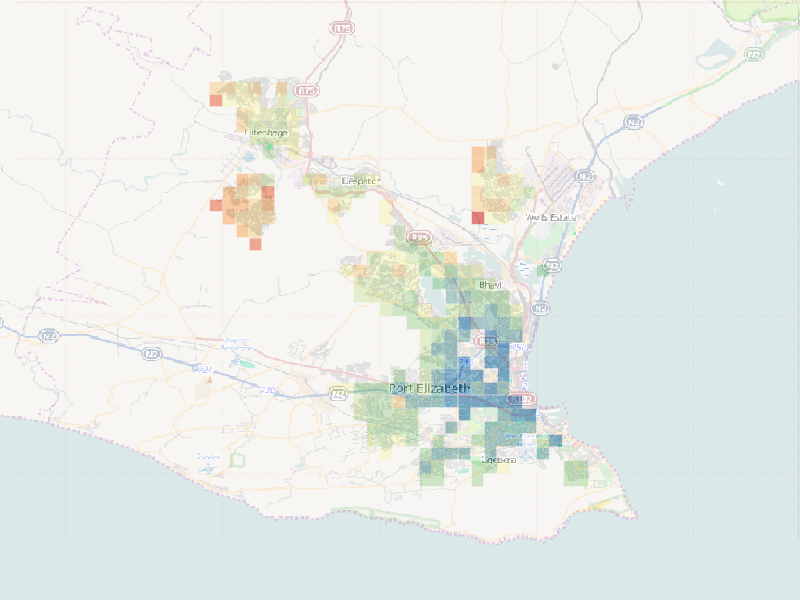
\includegraphics[width=1.\textwidth, angle=0]{extending/figures/accessibility/w_freeSpeed_snapshot.png} \end{center}

\createStandardInformation{accessibility}{\lstinline{RunAccessibilityExample} class}{accessibility}{\citet{NicolaiNagel2012HiResAccessibilityMethodInBook}}

% ##################################################################################################################
Note: This chapter draws on Nicolai Nagel

The term accessibility is used in the context of transport and infrastructure planning. The improvement of accessibility is often stated as a central goal of proposed transport or infrastructure schemes. Not in all contexts, however, in which accessibility is discussed, it is defined as a quantitative measure. First approaches to the quantitative computation of accessibilities appear to have been undertaken at the latest in the 1950s (cite Hansen ????????????). It is notable that the development of gravity models, which have since then been the most prominent and widely-applied type of destination choice models, has originally been intertwined with quantitative approaches to accessibility analysis (cite Hansen ?????).

Today, methods to assess the quality of accessibility (cite BBSR, TUHH, TUM, Curtis, ... ??????????) are often used in superordinate planning procedures like regional planning, where a central goal is to provide citizens with a certain quality of access to various services. Curtis et al. (cite Curtis... ??????) also argue that accessibility-based analysis methods may be suitable to overcome the deficits that traditional transport analysis methods possess in terms of analyzing transport policies that are not construction-based, e.g. transport demand management schemes.

\mnote{typology}
Depending on the concrete definition of quantitative accessibility measures, the explanatory power of the result varies widely. As pointed out by \citet{GeursRitsema2001AccessibilityMeasures} (\citep[see also][]{Geurs2004AccessibilityReview}), quantitative indicators can rely on the following approaches:
%
\begin{enumerate}
\item An \textbf{activity-based} or \textbf{land-use-based} approach focuses on
the distribution of possible activity locations (land use). One can, for instance,
base calculations on the number and spatial distribution of activity opportunities
like shopping locations or workplaces within a certain distance.
%
\item An \textbf{in\-fra\-struc\-ture-based} or \textbf{transport-based} approach takes into account the effort to travel from a given origin to a given destination and 
can be based on performance characteristics of the transport system, e.g. the
average speed by mode at certain locations. If one considers, for instance, the
number of shopping locations or workplaces under a defined travel time threshold,
the activity-based and the infrastructure-based approaches can be combined.
%
\item A \textbf{temporal} component, which considers the availability of activities at different times-of-day, may be added.
%
\item An \textbf{individual} approach to accessibility computations can be
obtained by addressing different needs and opportunities of different socio-economic groups, \eg different income groups.
%
\item A \textbf{utility-based} measurement of accessibility reflects the
(economic) benefits, as the maximum expected utility, that someone gains
from access to spatially distributed opportunities
\citep{GeursRitsema2001AccessibilityMeasures,deJongEtAl2007LogsumTRA}. The
typical example is the logsum term, which is discussed further below.
\end{enumerate}
%
%%%%%%%%%%%%%%%%%%%%%%%%%%%%%%%%%%%%%%%%%%%%%%%%%%%%%%%%%%%%%%
%
\mnote{Portfolio of opportunities}
Established and frequently applied approaches to accessibility analyses often calculate travel times to the next facility that offers a particular type of service (e.g. travel time to the next airport or next hospital, e.g. BBSR (\url{http://www.bbsr.bund.de/BBSR/DE/Raumbeobachtung/UeberRaumbeobachtung/Komponenten/Erreichbarkeitsmodell/erreichbarkeitsmodell_node.html}). ) and define this travel time as the accessibility (OR SAY use this as a proxy for accessibility....????).

While giving useful insights into the supply of the population with certain services, one can argue, however, that such approaches do not reflect the set of options, which a citizen can select from, very well. The measure will
arguably become more insightful, if not only the impedance to reach \textit{the nearest} facility serving a particular need is taken into account, but if instead a set of multiple reachable facilities serving the same need is considered. This is due to the fact, that different facilities of the same type may offer a given service in different qualities. Also, services may become more beneficent when combined with complementary services provided by another facility of the same type. For instance, a person wishing to make a holiday trip by airplane will likely take into account several airports in her/his vicinity when planning a journey instead of just looking at the flights offered from the nearest airport. Therefore, the accessibility to airports should be made dependent on the impedances to reach all of these airports instead of just the impedance to reach the nearest one. Facilities offering medical services may serve as another example. Only taking into account the nearest hospital may already be sufficient when looking at unsophisticated services like first aid, which can be assumed to be available at almost \textit{any} hospital. In other cases, however, the supply with medical services will be better represented by considering several hospitals in the vicinity because they are likely to offer different kinds of medical treatment that complement each other. Therefore, all reachable hospitals should be considered when calculating accessibilities of medical facilities instead of just taking into account the closest hospital. Only by including a set of potential locations, the approach becomes truly activity- or land-use-based in sense defined above.

In order to account for the multitude of facilities serving a given need, a (weighted) sum over the accessibilities of several facilities of a given type appears reasonable. The (quantitative) accessibility measure in the MATSim accessibility extension is of the mathematical form
\begin{equation}
A_i = g\Big( \sum_j a_j \, f(c_{ij}) \Big) \ ,
\label{eq:accessibility:basic}
\end{equation}
where the sum goes over all possible destinations (opportunities) $j$, $a_j$ is an indicator of the attractiveness of the opportunity, $c_{ij}$ is the generalized cost of travel to get from $i$ to $j$, $f(c)$ is an impedance function that typically decreases with increasing distance, and $g(.)$ is an arbitrary, but typically monotonically increasing, function.  That is, the accessibility at $i$ is computed from a weighted sum over all possible destinations, where the weight is the product of the destination's attractiveness and the ease to get there.

\mnote{ingoing vs. outgoing accessibility}
It is important to note that the above-defined measure quantifies how good the accessibility to certain services \textit{from} a given location $i$ is. This kind of accessibility may be referred to as "outgoing" accessibility, while a measure of "ingoing" accessibility would quantify how well a given location $i$ is accessible from other locations. \citet{NicolaiNagel2012HiResAccessibilityMethodInBook} discuss under which circumstances both measures are interchangeable.

\mnote{uncongested vs. congested network}
As mentioned above, accessibility computations are oftentimes based on travel times, which serve as an impedance measure. The calculation of the travel time can, however, vary. The most simple approach to calculate a travel time between two locations is measuring the Euclidian distance (beeline distance) between these two locations and then, by means of some kind of average speed, approximate the travel time between these two locations. This has obvious disadvantages as, for instance, the quality of the transport infrastructure or topographic obstacles are not considered. In this sense, such an approach would not meet the characteristics of an {in\-fra\-struc\-ture-based} or transport-based accessibility computation as pointed out above.

These disadvantages can be overcome by calculating actual travel routes and corresponding travel times on a network that represents the real-world transport infrastructure. While this calculation is obviously already possible by only considering transport supply, i.e. the transport network (potentially using a distinction of road types by speed; \eg BBSR (\url{http://www.bbsr.bund.de/BBSR/DE/Raumbeobachtung/UeberRaumbeobachtung/Komponenten/Erreichbarkeitsmodell/erreichbarkeitsmodell_node.html}). ), its expressiveness can be further increased by additionally taking into account transport demand as well. This is useful because the performance of the transport system is obviously dependent of the utilization of transport supply by transport demand. With increasing travel times, for instance, the accessibility of a given location may decrease. To be able to analyze such effects, a transport simulation which represents the interaction of transport supply and demand is needed. This is one major argument why it is reasonable to integrate an accessibility extension into the MATSim framework.

As a result, the accessibility computation can be made dependent upon time-of-day, which is useful in contexts were levels of transport demand varies significantly over the course of the day as, for instance, in contexts where pronounced morning and afternoon peaks exist. This way, accessibility changes related to transport policies and corresponding reaction of decision makers can be considered in a more comprehensive fashion.

\mnote{spatial resolution, zones vs. points}
In contrast to many other transport simulations, \gls{matsim} is not zone-based, but based on coordinates (see section ?????). Therefore, the accessibility computation within MATSim can also be conducted independent of any zonation system and, instead, be based on points or on a raster with arbitrary granularity. This avoids several issues that may arise if accessibility computations are based on zones (see \citep[e.g.,][]{NicolaiNagel2012HiResAccessibilityMethodInBook}) as it is done by other quantitative accessibility computations 
%
%\citep[e.g.][]{Curtis, BBSR , LiuZhu2004AccessibilityAnalyst} (?????)
\ah{temporarily commented out as it kills the continous integration: \url{http://ci.matsim.org:8080/view/All/job/MATSim-Book/ws/}}
%
(\url{http://www.bbsr.bund.de/BBSR/DE/Raumbeobachtung/UeberRaumbeobachtung/Komponenten/Erreichbarkeitsmodell/erreichbarkeitsmodell_node.html}). Being raster- or coordinate-based, the outcome of the MATSim accessibility computation can be considered as an accessibility field,
i.e.\ as a measure continuously varying in space, $A(x,y)$, where $x$ and $y$
are the coordinates. As is common in many areas of science, such
fields can be visualized by calculating the values on regular grid
points and using an averaging plotting routine (?????????). An example of such a visualization is shown in figure ????.

\mnote{econometric interpretation}
As pointed out by Curtis (????????????????) accessibilities can serve as an evaluation measure for transport policies. While most measures today rely on pure infrastructure characteristics (cite ??????????? look in ERAfrika-Antrag), accessibility indicators are a holistic measure, which explicitly observes the interrelationship between transport and land use.

To make the quantitative accessibility measure most expressive in terms of econometric evaluation (e.g. cost-benefit analyses), it seems sensible to adapt equation \ref{eq:accessibility:basic} as follows: $g(.) = \ln(.)$, $a_j = 1$, $f(c_{ij}) = e^{-c_{ij}}$, and $-c_{ij} = V_{ij}$. Thus, equation \ref{eq:accessibility:basic} becomes
\begin{equation}
A_i := \ln \sum_k e^{V_{ik}} \ ,
\label{eq:accessibility:logsum0}
\end{equation}
where $k$ goes over all possible destinations, and $V_{ik}$ is the
disutility of travel in order to get from location $i$ to location
$k$. Equation \ref{eq:accessibility:logsum0} is the so-called logsum term and has an econometric interpretation as the expected maximum utility \citep[e.g.][]{Ben-AkivaBook}. It can be derived as follows: Assume that the full utility of location $k$, seen from $i$, is $U_{ik} = V_{base} + V_{ik} + \epsilon_{ik}$, where $V_{base}$ is a constant base utility for doing the activity at any location, $V_{ik}$ is the systematic ($=$ observed) disutility to travel to location $k$, and $\epsilon_{ik}$ is a random term which picks up the randomness of the travel disutility and, more importantly, also the utility fluctuations around $V_{base}$.  Under the typical assumption that the $\epsilon_{ik}$ are independent and identically Gumbel-distributed random variables, the expectation value of $U_{ik}$ becomes
\begin{equation}
E(U_i) = E(\max_k U_{ik}) = \ln \sum_k e^{V_{ik}} + Const \equiv A_i + Const \ .
\end{equation}
$Const$ is an integration constant, which can be dropped as it is the same for all locations. $A_i$ may also be negative.

\mnote{functionings}
The concrete calculation of the accessibility $A_i$ of a given origin location $i$ to opportunity locations $k$ works as follows: The origin location $i$ and opportunity locations $k$ are assigned to a congested road network with time dependent travel times as it is simulated in MATSim. For every $i$ a so-called ``least cost path tree'' computation runs through the network and determines the best route, and thus the least negative travel utility $V_{ik}$, to each opportunity location $k$ by using Dijkstra's shortest path algorithm \citep{Dijkstra1959ShortestPath}. The best route from $i$ to $k$ depends on the given generalized cost such as link travel times or distances. Once the least cost path tree has explored all nodes, the resulting disutilities $V_{ik}$ for all opportunities are queried and the accessibility is calculated as stated in Equation~(\ref{eq:accessibility:logsum0}).


USAGE: controlerListener in MATSim; if various activities and various modes are considered, one such contoler listener is added for each combination


\mnote{computational aspects}
TODO: say something about computation characteristics

runtime optimization

\mnote{resolution}
resolution can in principal be increased infinitely. Because of the runtime optimization, computation time increases sub-linearly with resolution.

studies showed that no significant further insights can be gained by increasing the resolution beyond 100\,meters.

\mnote{other}
ADD: different modes, activities

ADD: transport/land-use interaction

automatic

microscopic

\mnote{data}
free data

the accessibility computation does not rely on specific local data, that need to be collected, prepared and processed. Instead, it relies on data form \gls{osm} (include link...?) which is openly and freely for every region in the world, and also has the same data format world-wide

\mnote{applicability, useability}




%Aufgabe des Staates: Grundversorgung der Bevölkerung
%Nötig: (Infrastruktur-)Maßnahmen bewerten
%Heute i.d.R. ausschließlich auf Basis verkehrs- und mobilitätsbezogener Maße
%Qualität der erreichbaren Angebote
%Nicht bewertet
%Mittels Durchschnittswerten bewertet
%Keine Aussage bzgl. etwaiger räumlicher und/oder sozialer Ungleichverteilungen
%Verteilungsmaße (z.B. generalisierter Gini-Koeffizient)
%Verortung unterversorgter Personen?
%Beitrag zur Verbesserung des Zugangs zum jeweiligen Angebot?





\section{Invocation}

\subsection{Minimal}

...



\subsection{Invocation as ``Script in Java''}

See \url{http://matsim.org/javadoc} $\to$ accessibility $\to$ \lstinline{RunAccessibility} class for an example.



% ##################################################################################################################

% Local Variables:
% mode: latex
% mode: reftex
% mode: visual-line
% TeX-master: "../../main"
% comment-padding: 1
% fill-column: 9999
% End: 
